% Author Vahid Partovi Nia
% Copyright Huawei Technologies
% Network Mind Team



\documentclass[12pt]{beamer}

\usetheme{Hannover}
\setbeamercolor{section in sidebar shaded}{fg=black}

\usecolortheme{beaver}
\beamertemplatenavigationsymbolsempty

%  \usebeamertemplate{navigation symbols}\hfill
%  \insertframenumber{}/\inserttotalframenumber}
  

\useoutertheme{sidebar}
\pgfdeclareimage[width=2.5\baselineskip]{institut-logo}{fig/mcgill_logo}
\setbeamertemplate{footline}
{\raisebox{-2ex}{\pgfuseimage{institut-logo}}
%  \hfill
\hspace{5cm}
  \usebeamertemplate{navigation symbols}
  \insertframenumber{}/\inserttotalframenumber
  \hspace{3.8cm}
YCBS255
}
%\setbeamertemplate{sidebar right}{}
  
\setbeamercolor{block title}{fg=darkred}
\setbeamercolor{local structure}{fg=darkred}

\setbeamercolor{palette sidebar secondary}{fg=darkgray, bg=white}



\usefonttheme{professionalfonts} % using non standard fonts for beamer


\makeatletter
\beamer@nav@subsectionstyle{hide/hide/hide}
\makeatother

\titlegraphic{
\includegraphics[width=2cm]{fig/mcgill_logo}}




\usepackage{listings}
\usepackage{xcolor}
\def \y {\mathbf y}
\def \X {\mathbf X}
\def \A {\mathbf A}
\def \t {^\top}
\def \inv {^ {-1}}
\def \x {\mathbf x}
\def \bbeta {\boldsymbol \beta}
\def \eeps {\boldsymbol \varepsilon}
\def \TV {\mathrm{TV}}
\def \Radio {\mathrm{Radio}}
\def \Newspaper {\mathrm{Newspaper}}
\def \Sales {\mathrm{Sales}}
\def \Balance {\mathrm{Balance}}
\def \Default {\mathrm{Default}}

\definecolor{capri}{rgb}{0.0, 0.75, 1.0}
\definecolor{darkcyan}{rgb}{0.0, 0.55, 0.55}
\definecolor{deepfuchsia}{rgb}{0.76, 0.33, 0.76}
\begin{document}

% no title and no author on sidebar
\title[]{Classification}   
\author[]{Vahid Partovi Nia} 
\institute{Lecture 03}
\date{6 November 2018}


\makeatletter
  \begin{frame}[plain]
    \hspace*{-\beamer@leftsidebar}%
    \advance\textwidth by \beamer@leftsidebar\relax
    \beamer@leftsidebar=\z@
    \begin{minipage}{\textwidth}\par%
      \maketitle
    \end{minipage}
  \end{frame}
  \makeatother



\frame{\frametitle{Outline}\tableofcontents} 

\setbeamertemplate{sidebar left}[sidebar theme]


\section{Terminology}



\frame{\frametitle{Supervised Learning}
\begin{itemize}
\item Regression: $y$ is continuous
\item Classification: $y$ is discrete
\end{itemize}
}


\section{Default dataset}
\frame{\frametitle{Default dataset}
Default:  After you’ve failed to make a payment on your credit card for 180 days, your issuer assumes you’re probably never going to. The issuer closes your card, write off what you owe as bad debt, and sells your account to a collection agency.
\begin{itemize}
\item  $y$: default on credit card `` No=0" or  ``Yes=1" 
\item $x_1$: Income
\item $x_2$: Credit Balance 
\end{itemize}
}


\frame{\frametitle{Scatterplot}
\begin{center}
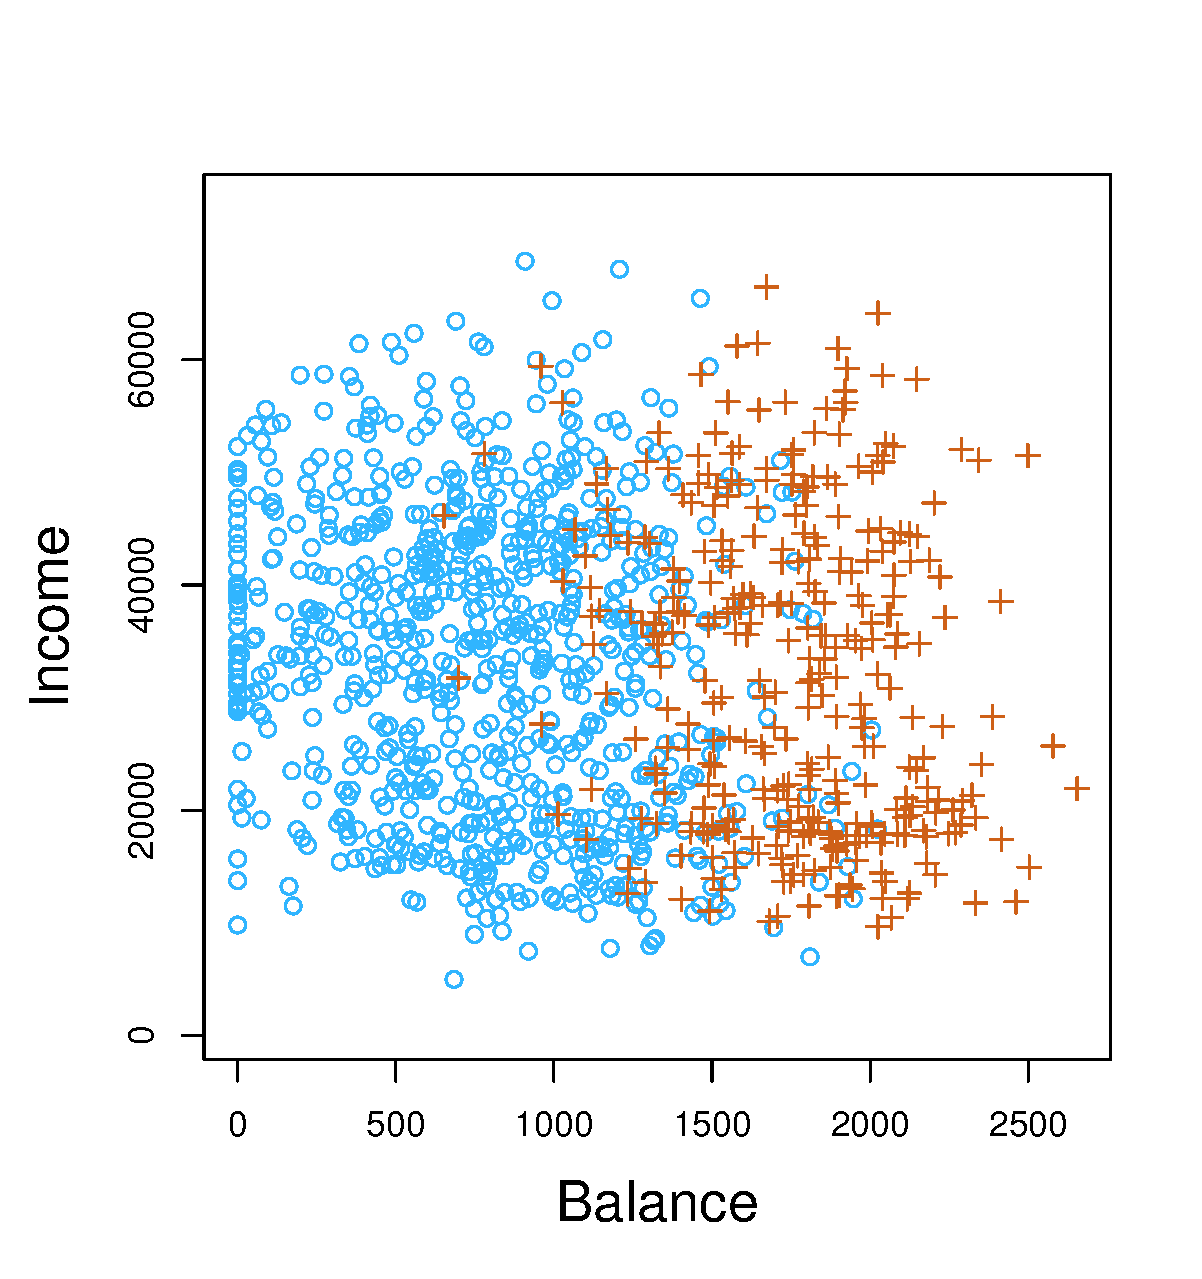
\includegraphics[width=0.6\textwidth]{fig/4-1a}
\end{center}
\begin{itemize}
\item No = 0 =  {\color{capri} {O}}
\item Yes = 1 = {\color{orange} {+}}
\end{itemize}
}


\frame{\frametitle{Boxplot}
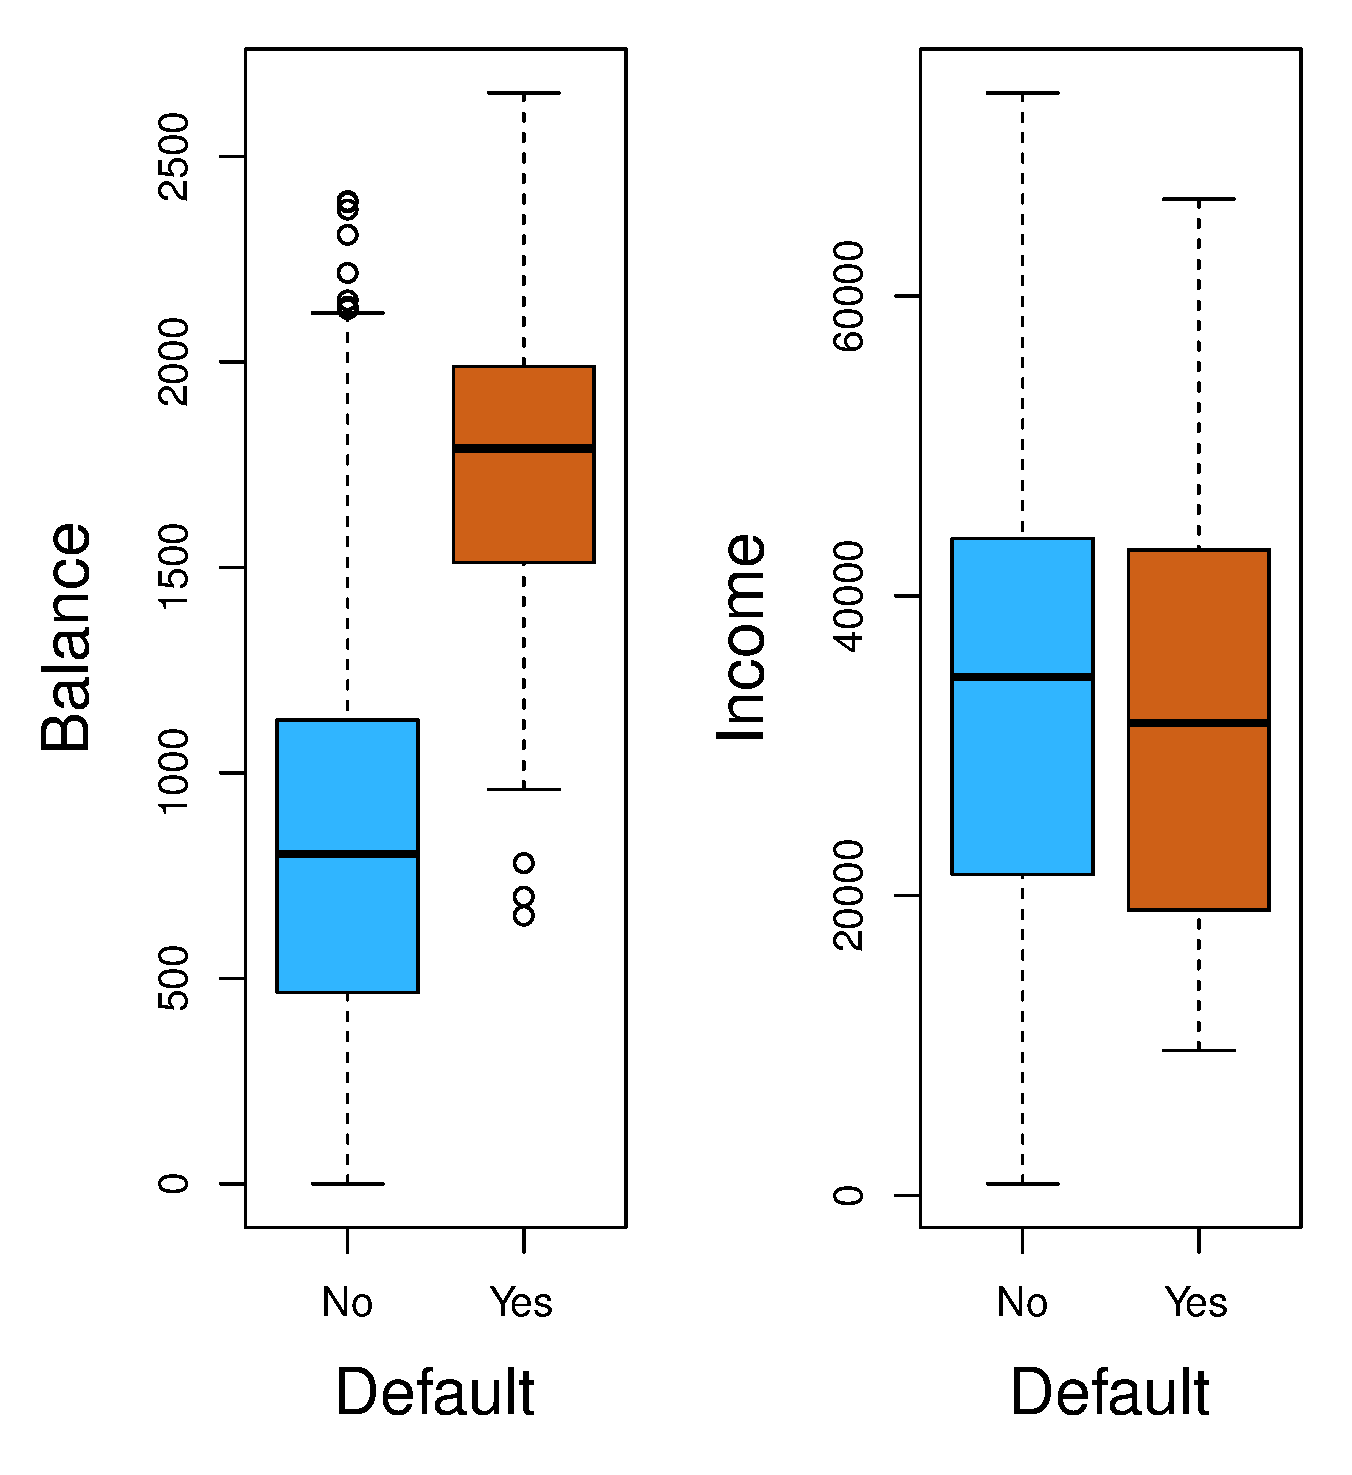
\includegraphics[width=0.7\textwidth]{fig/4-1b}
}


\frame{\frametitle{Regression for Classification}
Simplify: let's focus only on ``Balance" as the predictor of ``default".
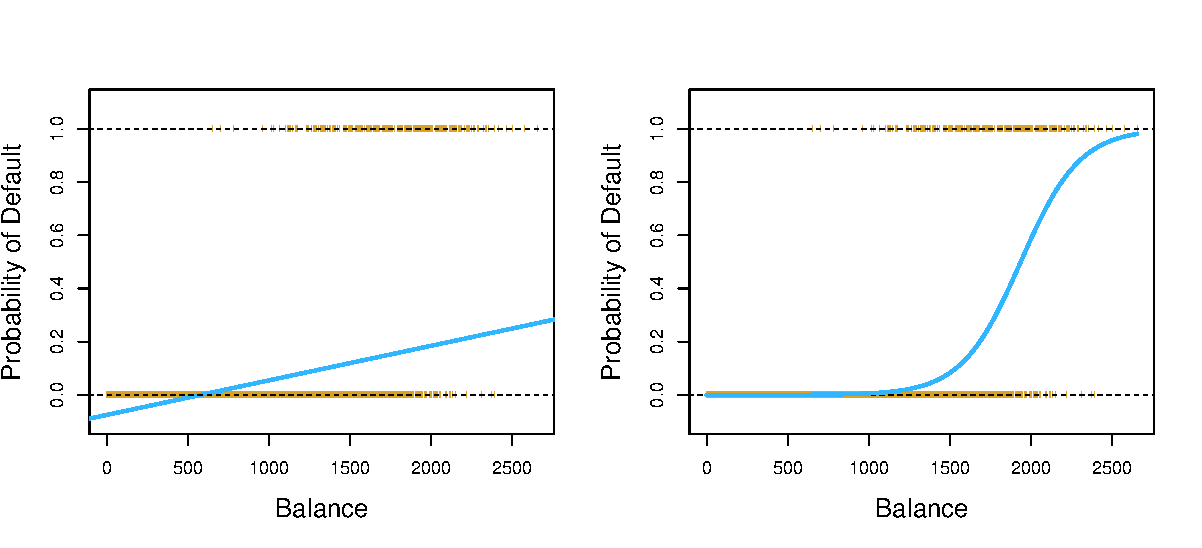
\includegraphics[width=\textwidth]{fig/4-2}
}

\frame{\frametitle{}
\begin{eqnarray*}
y_i &=& \beta_0 +\varepsilon_i \\
\varepsilon_i &\sim& N(0,\sigma^2)
\end{eqnarray*}
This means
\begin{eqnarray*}
y_i &\sim& N(\beta_0, \sigma^2) \\
\end{eqnarray*}
$$y_i \sim B(p_0) = \left\{ \begin{array}{c c} y_i=1 & \textrm{with probability } p_0  \\  y_i=0 & \textrm{with probability } 1-p_0  \end{array} \right. $$
One may define 
\begin{itemize}
\item $p_0 = p(\beta_0) = {1  \over {1+e^{\beta_0}}} $
\item For $\beta_0 \in \mathbb R,$ always $0 < p_0 < 1.$ 
\end{itemize}
}

\frame{\frametitle{Simple Logistic Regression}
$$\tiny\Default_i \mid \Balance_i \sim B(p_i) = \left\{ \begin{array}{c c} \Default_i=1 & \textrm{with probability } p_i  \\  \Default_i=0 & \textrm{with probability } 1-p_i  \end{array} \right. $$
\begin{itemize}
\item $p_i = p(\beta_0+\beta_1 \Balance_i) = {1  \over {1+e^{\beta_0 + \beta_1 \Balance_i}}} $
\item For $(\beta_0,\beta_1) \in \mathbb R^2,$ always $0 < p_i < 1.$ 
\end{itemize}
}

\frame{\frametitle{Simple Regression}
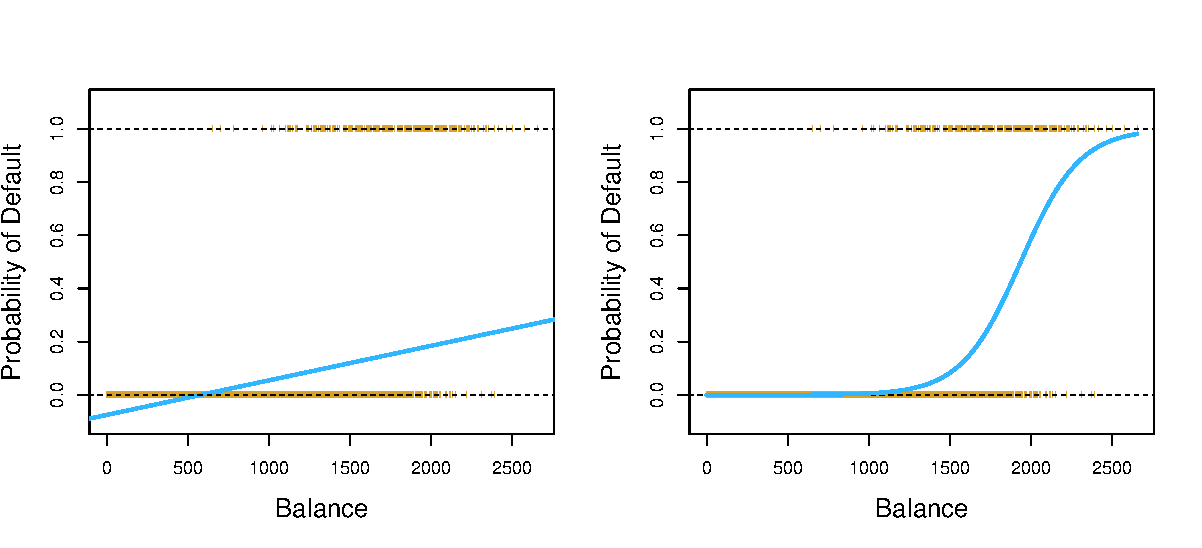
\includegraphics[width=\textwidth]{fig/4-2}
\begin{eqnarray*}
p_i = \beta_0+\beta_1 x_i \quad \quad \quad \quad \quad \quad  p_i &=& {1  \over {1+e^{\beta_0 + \beta_1 \Balance_i}}}\\
\log\left( {p_i \over 1-p_i}\right) &=& \beta_0 + \beta_1 \Balance_i
\end{eqnarray*}
}

\begin{frame}[fragile]
\tiny
\begin{lstlisting}
import pandas as pd
path='data/'
filename = path+'Default.xlsx'
default_data = pd.read_excel(filename)
\end{lstlisting}
\pause
\begin{lstlisting}
default_data['default_factor'] = default_data.default.factorize()[0]
default_data.head()
\end{lstlisting}
\pause
\begin{lstlisting}
from sklearn.linear_model import LogisticRegression

X = default_data[['balance']]
y = default_data['default_factor']
\end{lstlisting}

\begin{lstlisting}
lr = LogisticRegression()
lr.fit(X, y)
\end{lstlisting}
\end{frame}

\begin{frame}[fragile]\frametitle{Predict}
Predict the probability of Default = 'Yes' for $\Balance =  1500$ and $\Balance = 2000$
Implement simple logistic regression on credit data 

\pause
{\tiny 
\begin{lstlisting}
import numpy as np
X_pred = np.array([1500, 2000]).reshape(-1,1)
print(lr.predict_proba(X_pred))
\end{lstlisting}}
\end{frame}


\frame{\frametitle{Multiple Logistic Regression}
\begin{itemize}
\item  $y$: default on credit card `` No=0" or  ``Yes=1" 
\item $x_1$: Income
\item $x_2$: Credit Balance 
\end{itemize}
}


\frame{\frametitle{Coefficient interpretation}
Implement simple logistic regression on credit data 
}

\section{LDA}

\frame{\frametitle{Linear Disceiminant}
\begin{itemize}
\item Logistic Regression models $\Default_i \mid \Balance_i$
\item Linear Discriminant models $\Balance_i \mid \Default_i$
\end{itemize}
}

\frame{\frametitle{Linear Discriminant}
\begin{itemize}
\item $\Balance_i\mid {\color{darkcyan} \Default_i=0}\sim N(\beta_0, \sigma^2)$
\item $\Balance_i\mid {\color{deepfuchsia} \Default_i=1} \sim N(\beta_1, \sigma^2)$
\end{itemize}
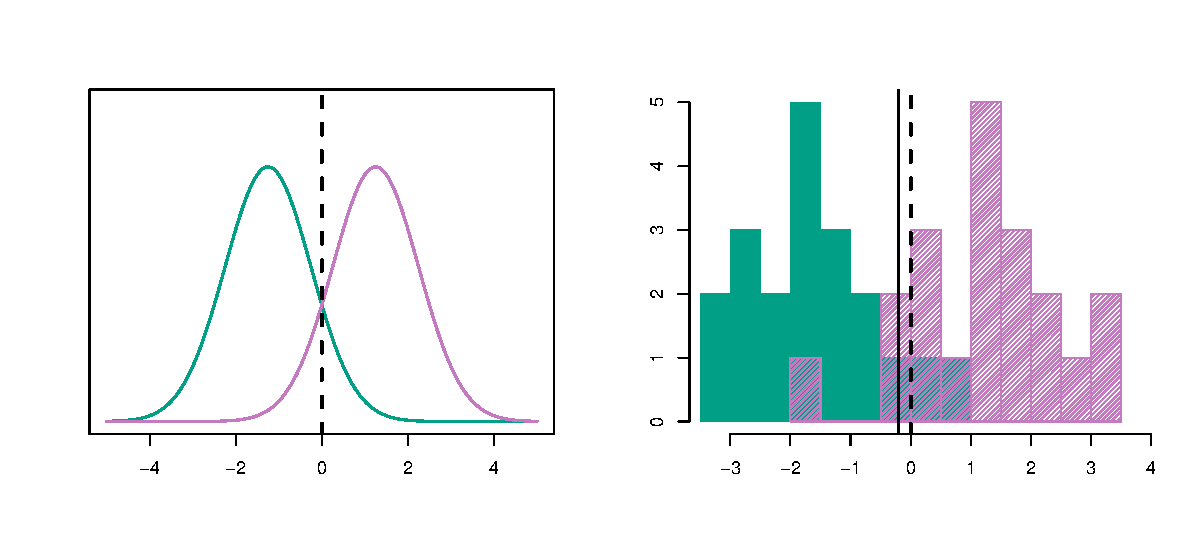
\includegraphics[width=\textwidth]{fig/4-4}
}

\begin{frame}[fragile]\frametitle{LDA }
\tiny
\begin{lstlisting}
from sklearn.discriminant_analysis import LinearDiscriminantAnalysis
X = default_data[['balance']]
y = default_data['default_factor']
lda = LinearDiscriminantAnalysis()
lda.fit(X,y)
\end{lstlisting}
\pause
\begin{lstlisting}
X_pred = np.array([1500, 2000]).reshape(-1,1)
print(lda.predict_proba(X_pred))
\end{lstlisting}

%\begin{lstlisting}
%\end{lstlisting}

\end{frame}

\section{QDA}
\frame{\frametitle{Quadratic Discriminant}
\begin{itemize}
\item $\Balance_i\mid {\color{darkcyan} \Default_i=0}\sim N(\beta_0, \sigma_0^2)$
\item $\Balance_i\mid {\color{deepfuchsia} \Default_i=1} \sim N(\beta_1, \sigma_1^2)$
\end{itemize}
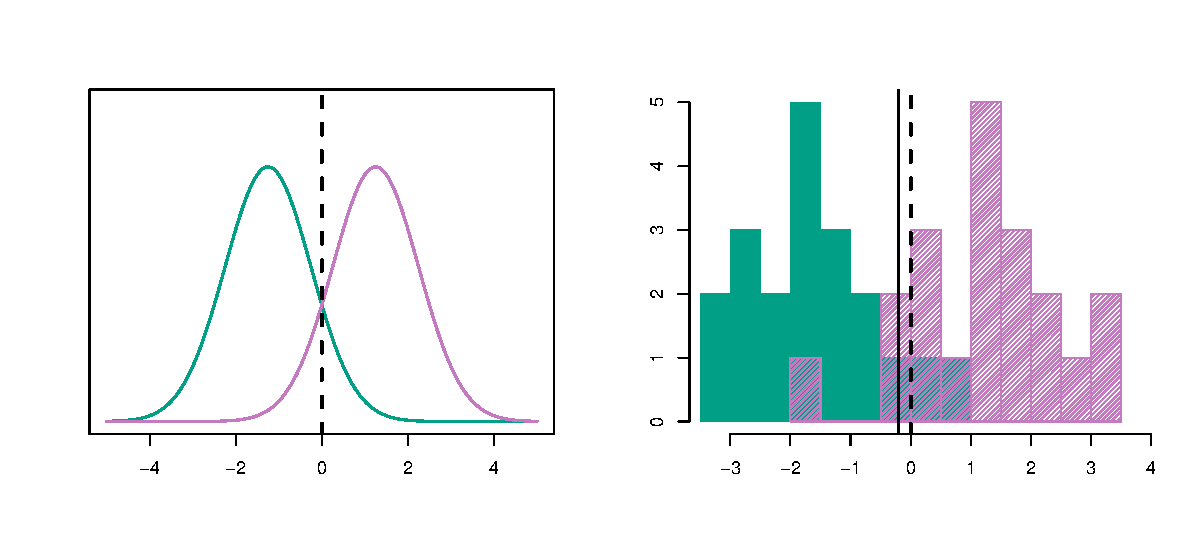
\includegraphics[width=\textwidth]{fig/4-4}
}

\begin{frame}[fragile]\frametitle{QDA }
\tiny
\begin{lstlisting}
from sklearn.discriminant_analysis import QuadraticDiscriminantAnalysis
X = default_data[['balance']]
y = default_data['default_factor']
qda = QuadraticDiscriminantAnalysis()
qda.fit(X,y)
\end{lstlisting}
\pause
\begin{lstlisting}
X_pred = np.array([1500, 2000]).reshape(-1,1)
print(qda.predict_proba(X_pred))
\end{lstlisting}

%\begin{lstlisting}
%\end{lstlisting}
\end{frame}


\frame{\frametitle{statsmodels}
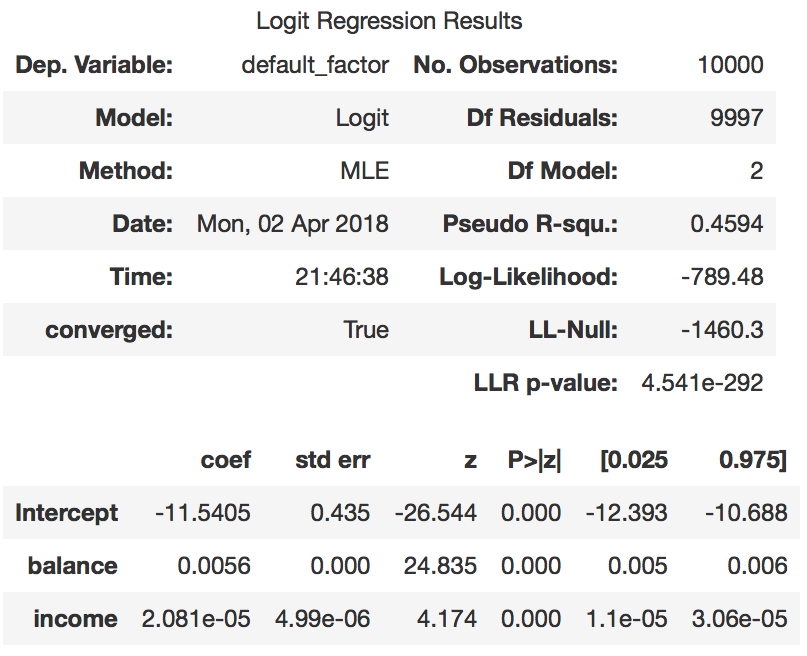
\includegraphics[width=0.5\textwidth]{fig/logistic}
}


%\frame{\frametitle{}
%\includegraphics[width=0.5\textwidth]{fig/}
%}
%\frame{\frametitle{}
%\includegraphics[width=0.5\textwidth]{fig/}
%}
%\frame{\frametitle{}
%\includegraphics[width=0.5\textwidth]{fig/}
%}
%\frame{\frametitle{}
%\includegraphics[width=0.5\textwidth]{fig/}
%}
%\frame{\frametitle{}
%\includegraphics[width=0.5\textwidth]{fig/}
%}
%\frame{\frametitle{}
%\includegraphics[width=0.5\textwidth]{fig/}
%}
%
%
%
%

\end{document}
